
\documentclass[sigconf]{acmart}
\AtBeginDocument{%
  \providecommand\BibTeX{{%
    Bib\TeX}}}

\usepackage{lipsum}

\setcopyright{acmlicensed}
\copyrightyear{2018}
\acmYear{2018}
\acmDOI{XXXXXXX.XXXXXXX}
\acmConference[Conference acronym 'XX]{Make sure to enter the correct
  conference title from your rights confirmation email}{June 03--05,
  2018}{Woodstock, NY}

\acmISBN{978-1-4503-XXXX-X/2018/06}

\begin{document}

\title{CSE331 - Assignment \#1}

\author{\textcolor{blue}{Hangyeol Choi (20191315)}}
\affiliation{%
  \institution{UNIST}
  \country{South Korea}
}
\email{whwhsu445@unist.ac.kr}

\renewcommand{\shortauthors}{\textcolor{blue}{Choi et al.}}



\settopmatter{printacmref=false} % Removes citation block in the first page
\renewcommand\footnotetextcopyrightpermission[1]{} % Removes footnote with conference info



\maketitle


\section{PROBLEM STATEMENT}
Efficient sorting is a fundamental problem in computer science, with applications spanning data processing, database indexing, and algorithmic optimization. Over decades of research, a wide spectrum of sorting algorithms has emerged—ranging from simple comparison-based methods such as bubble sort and insertion sort to advanced hybrid techniques like introsort and timsort used in modern programming libraries.

Despite the extensive body of literature, the practical performance of sorting algorithms often depends on specific data characteristics, including the degree of order, size, and data distribution. In contemporary computing environments where large-scale datasets are prevalent, it becomes crucial to understand the trade-offs between algorithmic complexity, stability, and real-world efficiency.

This project aims to systematically implement and evaluate both classical and modern sorting algorithms. The study includes six traditional comparison-based sorting algorithms—merge sort, heap sort, bubble sort, insertion sort, selection sort, and quick sort—alongside six modern sorting techniques such as library sort, timsort, comb sort, and introsort. Each algorithm will be implemented from scratch or pseudo-coded, and will be analyzed in terms of its theoretical complexity and practical behavior.

To provide a comprehensive performance comparison, we generate diverse input datasets, ranging from fully sorted to completely random, and measure execution time, memory usage, and stability across varying input sizes from 1,000 to 1,000,000 elements. Each experiment is repeated multiple times to ensure statistically meaningful results.

Through this study, we seek to answer the following questions:

How do classical and modern sorting algorithms compare in terms of efficiency and resource usage?

In what scenarios do modern hybrid approaches outperform traditional methods?

\section{BASIC SORTING ALGORITHMS}
\subsection{Merge Sort}
Merge Sort is a classic sorting algorithm based on the Divide and Conquer strategy. It works by dividing the entire array in half, recursively sorting each half, and then merging them. This approach has a structural advantage by breaking down the problem into smaller units, and since the division process occurs consistently as a binary tree of depth$log(n)$, it guarantees a stable time complexity.

The time complexity of merge sort is $O(nlog(n))$ in all cases. This is because the input array of size n is divided$log(n)$ times (as shown by a division tree of height$log(n)$), and every element must be compared during the merge process, which takes $O(n)$ time. However, since merge sort requires additional arrays during the merging process, its space complexity is $O(n)$, which can be relatively inefficient.

\begin{figure}[t]
\centering
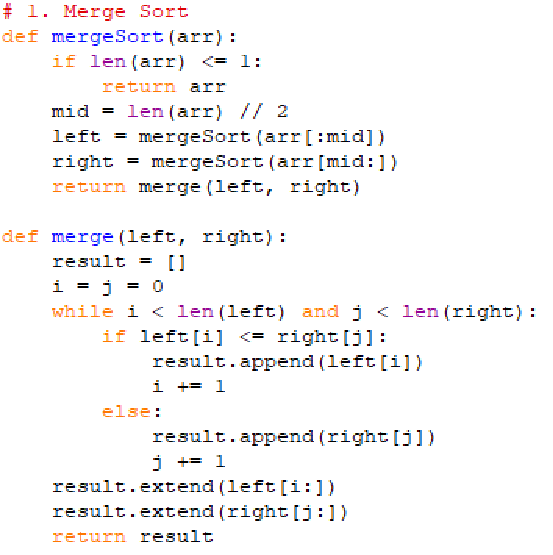
\includegraphics[width=0.85\linewidth]{figures/001.pdf}
\vspace{-0.3cm}
\caption{Merge Sort Code}  
\vspace{-0.35cm}
\label{fig:proportion}
\end{figure}

In this code, the mergeSort function recursively divides the array, and the merge function merges two sorted arrays into one. Specifically, the condition $(left[i] <= right[j])$ ensures that if two elements are equal, the one from the left subarray is chosen first, thus maintaining stability. The use of a new result list for merging confirms that this is not an in-place sort and requires extra memory.
\subsection {Heap Sort}
Heap Sort is a sorting algorithm that uses the heap data structure, which is based on a complete binary tree. It transforms the input array into a max-heap, moves the root (the maximum value) to the end of the array, and then repeatedly rebuilds the heap for the remaining elements to complete the sorting.

The time complexity for building the heap is $O(n)$, and the sorting process takes $O(nlog(n))$ (as each heapify call takes $O(log(n))$, so the overall time complexity is $O(nlog(n))$ in the best, average, and worst cases. Since no additional memory is used, the space complexity is $O(1)$. Heap sort is known for consistent performance among comparison-based sorting algorithms.
However, because heapify only compares values and not the original order, the relative order of equal elements can change, making heap sort unstable.

\begin{figure}[t]
\centering
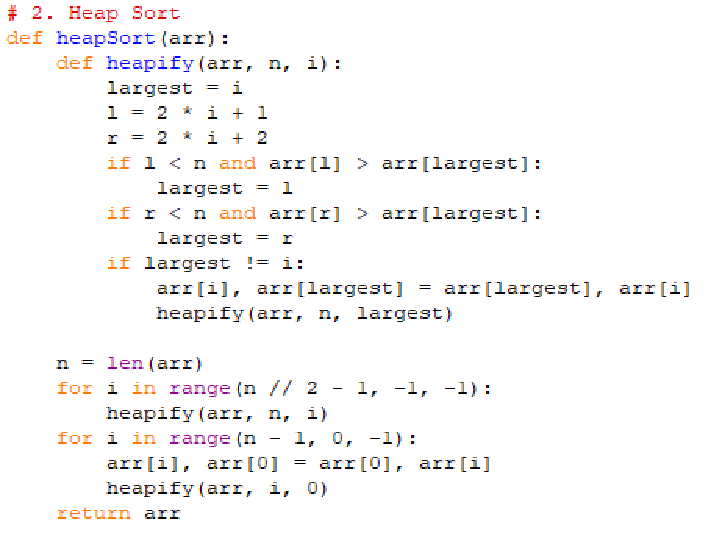
\includegraphics[width=0.85\linewidth]{figures/002.pdf}
\vspace{-0.3cm}
\caption{Heap Sort Code}  
\vspace{-0.35cm}
\label{fig:proportion}
\end{figure}

This implementation uses a heapify function to maintain the heap structure. It first builds a heap using a bottom-up approach (with for i in range$(\left\lfloor \frac{n}{2} \right\rfloor - 1, -1, -1)$), then repeatedly extracts the root and restores the heap. The code clearly demonstrates heap sort's structure and its complexity analysis.


\subsection{Bubble Sort}
Bubble Sort is a simple comparison-based sorting algorithm that repeatedly compares and swaps adjacent elements if they are in the wrong order. The algorithm "bubbles" the largest (or smallest) value to the end of the array during each pass.

Its design is intuitive and easy to implement. It can perform better when the input is nearly sorted, as fewer comparisons and swaps are needed.

The time complexity varies depending on the initial order:

Worst case (reversed order): $O(n^2)$

Average case: $O(n^2)$

Best case (already sorted): $O(n)$, if early termination optimization is applied using a flag to detect no swaps.

Space complexity is $O(1)$ since no extra memory is used. Bubble sort is stable, as it only swaps adjacent elements and maintains the relative order of equal values.

\begin{figure}[t]
\centering
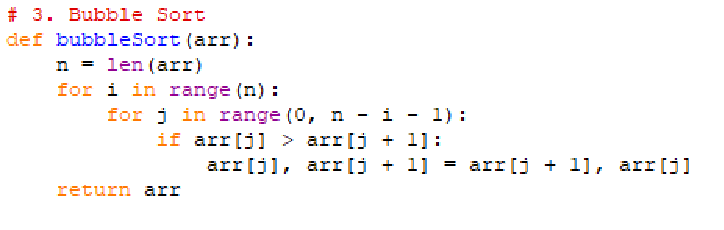
\includegraphics[width=0.85\linewidth]{figures/003.pdf}
\vspace{-0.3cm}
\caption{Bubble Sort Code}  
\vspace{-0.35cm}
\label{fig:proportion}
\end{figure}

This implementation uses two nested loops, comparing arr[j] and arr[j+1] and swapping when needed. This reflects bubble sort's core principle: pushing the largest element to the unsorted region's end on each pass.

\subsection{Insertion Sort}
Insertion Sort builds a sorted array one element at a time by inserting each new element into its appropriate position in the sorted portion. It's similar to how we sort cards in our hands while playing a card game.

It's simple and works efficiently for nearly sorted data.

Time complexity depends on the input:

Worst case (reverse order): $O(n^2)$

Average case: $O(n^2)$

Best case (already sorted): $O(n)$

Space complexity is $O(1)$, and it is stable because equal elements retain their relative order when using a "greater than" condition for comparisons.

\begin{figure}[t]
\centering
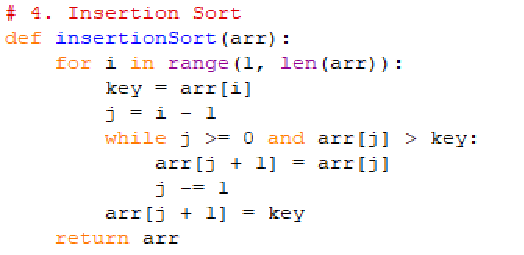
\includegraphics[width=0.85\linewidth]{figures/004.pdf}
\vspace{-0.3cm}
\caption{Insertion Sort Code}  
\vspace{-0.35cm}
\label{fig:proportion}
\end{figure}

This implementation starts at index 1 and moves backward through the sorted portion of the array to insert the key into the correct position. Larger elements are shifted right to make space for insertion.

\subsection{Selection Sort}
Selection Sort repeatedly selects the smallest (or largest) element from the unsorted part of the array and moves it to the front. It's simple and intuitive, often used for educational purposes.

Its time complexity is $O(n^2)$ in all cases (best, average, worst) because it performs $\frac{n(n-1)}{2}$ comparisons regardless of the input's order.
However, it performs only up to n-1 swaps, making it more efficient in terms of data movement compared to bubble or insertion sort.

Selection sort is not stable, because during the swapping process, the relative order of equal elements can change.

\begin{figure}[t]
\centering
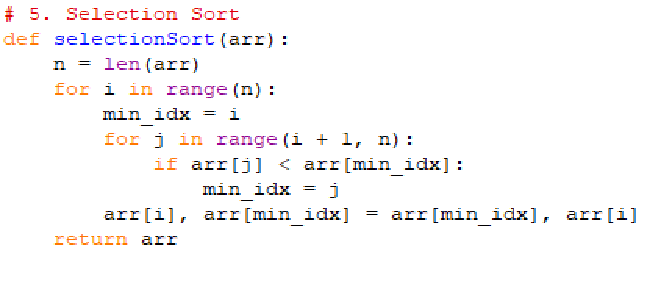
\includegraphics[width=0.85\linewidth]{figures/005.pdf}
\vspace{-0.3cm}
\caption{Selection Sort Code}  
\vspace{-0.35cm}
\label{fig:proportion}
\end{figure}

The code loops through the array, finds the index of the smallest element in the unsorted part, and swaps it with the first unsorted element. This process continues until the entire array is sorted.
\subsection{Quick Sort}
Quick Sort is an efficient sorting algorithm using the Divide and Conquer approach. It selects a pivot and partitions the array into two subarrays one with elements less than the pivot and the other with elements greater than the pivot then recursively applies quick sort to the subarrays.

Its time complexity varies:

Worst case: $O(n^2)$, when the array is already sorted or reversed.

Average case: $O(nlog(n))$, assuming good pivot choices.

Best case: $O(nlog(n))$, when the pivot perfectly divides the array.

Quick sort is not stable, since equal elements can change order during partitioning.

Space complexity is $O(n)$ due to recursive calls, though it doesn't use extra arrays like merge sort.

\begin{figure}[t]
\centering
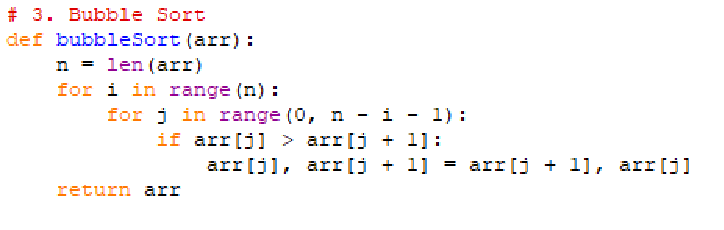
\includegraphics[width=0.85\linewidth]{figures/006.pdf}
\vspace{-0.3cm}
\caption{Quick Sort Code}  
\vspace{-0.35cm}
\label{fig:proportion}
\end{figure}

This implementation chooses the pivot as the middle element $(pivot = arr[len(arr) // 2])$. While this usually results in good performance, it can lead to poor results on sorted or reversed arrays. Alternative pivot selection methods (randomized, first, or last element) can help avoid the worst-case behavior.

\section{ADVANCED SORTING ALGORITHMS}
\lipsum[1]

\section{EXPERIMENTAL RESULTS AND ANALYSIS}
\lipsum[1]


% \bibliographystyle{ACM-Reference-Format}
% \bibliography{reference}

\end{document}
